% --------------------------------------------------------------
% This is all preamble stuff that you don't have to worry about.
% Head down to where it says "Start here"
% --------------------------------------------------------------
 
\documentclass[12pt]{article}
 
\usepackage[margin=1in]{geometry} 
\usepackage{amsmath,amsthm,amssymb}
\usepackage{gensymb}
\usepackage{graphicx}
 
\newcommand{\N}{\mathbb{N}}
\newcommand{\Z}{\mathbb{Z}}
 
\newenvironment{theorem}[2][Theorem]{\begin{trivlist}
\item[\hskip \labelsep {\bfseries #1}\hskip \labelsep {\bfseries #2.}]}{\end{trivlist}}
\newenvironment{lemma}[2][Lemma]{\begin{trivlist}
\item[\hskip \labelsep {\bfseries #1}\hskip \labelsep {\bfseries #2.}]}{\end{trivlist}}
\newenvironment{exercise}[2][Exercise]{\begin{trivlist}
\item[\hskip \labelsep {\bfseries #1}\hskip \labelsep {\bfseries #2.}]}{\end{trivlist}}
\newenvironment{problem}[2][Problem]{\begin{trivlist}
\item[\hskip \labelsep {\bfseries #1}\hskip \labelsep {\bfseries #2.}]}{\end{trivlist}}
\newenvironment{question}[2][Question]{\begin{trivlist}
\item[\hskip \labelsep {\bfseries #1}\hskip \labelsep {\bfseries #2.}]}{\end{trivlist}}
\newenvironment{corollary}[2][Corollary]{\begin{trivlist}
\item[\hskip \labelsep {\bfseries #1}\hskip \labelsep {\bfseries #2.}]}{\end{trivlist}}
 
\begin{document}
\providecommand{\e}[1]{\ensuremath{\times 10^{#1}}}
% --------------------------------------------------------------
%                         Start here
% --------------------------------------------------------------
 
\title{HW 2}%replace X with the appropriate number
\author{Levon Dovlatyan, SI: 24451582\\ %replace with your name
E45} %if necessary, replace with your course title
 
\maketitle
 
\begin{problem}{2.9} %You can use theorem, exercise, problem, or question here.  Modify x.yz to be whatever number you are proving
A copper penny has a mass of 2.60 g. Assuming pure copper, how much of this mass is contributed by \textbf{(a)} the neutrons in the copper nuclei and \textbf{(b)} electrons?
\end{problem}
 
\textbf{(a)} Cu-63 has 29 protons and 34 neutrons. The mass of a copper atom is,
\begin{align*}
\frac{63.546 \, g}{1 \, mole} = \frac{63.546 \,g}{6.022 \e{23} \, atoms} = \frac{1.055 \e{-22} \,g}{Cu \,\,atom}
\end{align*}

Now find the mass percent of neutrons in a copper atom \\ \\
$\frac{34 \,\text{neutrons} * 1.6749 \e{-24} g}{1 \, neutron} = 5.695 \e{-23} \, g \Rightarrow \frac{5.695 \e{-23} \, g/\text{Cu}}{1.055 \e{-22} \, g/\text{Cu} } = 53.98\%$ neutron mass in Cu \\ \\
Finally, $2.60 \, g * 0.5398 = 1.40 \, g$ of neutrons. \\

\textbf{(b)} Same idea fo electrons. Find the mass of 29 electrons and compare to Cu atom mass.
\begin{align*}
29 \,\text{electrons} * \frac{9.11 \e{-28} \, g}{1 \,\text{electron}} = 2.64 \e{-26} \, g \\
\frac{2.64 \e{-26} \,g/Cu}{1.055 \e{-22} \, g/Cu} = 2.50 \e{-4} \, \% \text{electron mass in Cu}
\end{align*}
Finally, $2.60 \, g * 2.50 \e{-4}= 6.51 \e{-4} \, g$ of electrons. \\

\begin{problem}{2.13}
Make an accurate plot of $F_c$ versus a (comparable to that shown in Figure 2.6) for an $Mg^{2+} -O^{2-}$ pair. Consider the range of a from 0.2 to 0.7 nm.
\end{problem}

Using the equation $F_c = \frac{-K}{a^2}$ where $K = k_0Z_1Z_2q^2$ and $Z_1 = +2, Z_2 = -2.$
\begin{center}
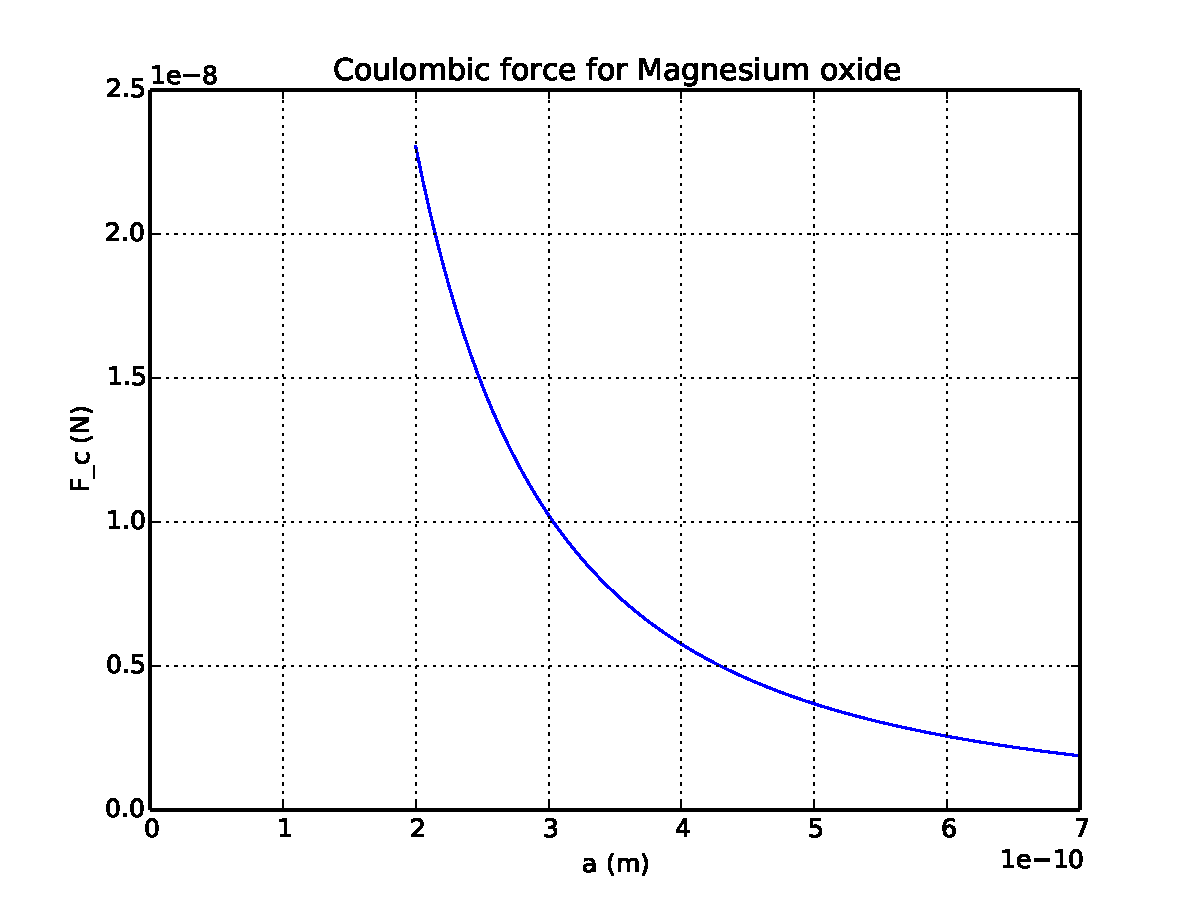
\includegraphics[width=250pt]{graph_p2_13.pdf}
\end{center}

\begin{problem}{2.33}
The first step in the formation of phenolformaldehyde, a common phenolic polymer, is shown in Figure 12.6. Calculate the net reaction energy (per mole) for this step in the overal polymerization reaction.
\end{problem}

initially the $C = O$ bond is broken and two $C - H$ bonds are formed.
\begin{align*}
C = C \rightarrow 2\,C-H \\
535 \text{kj/mole} \rightarrow 2(435 \text{kJ/mole}) \\
(870 - 535) \text{kJ/mole} = 335 \text{kJ/mole}
\end{align*}

\begin{problem}{2.46}
Plot the bond length of the metals in the long row of metallic elements (K to Ga).
\end{problem}

\begin{center}
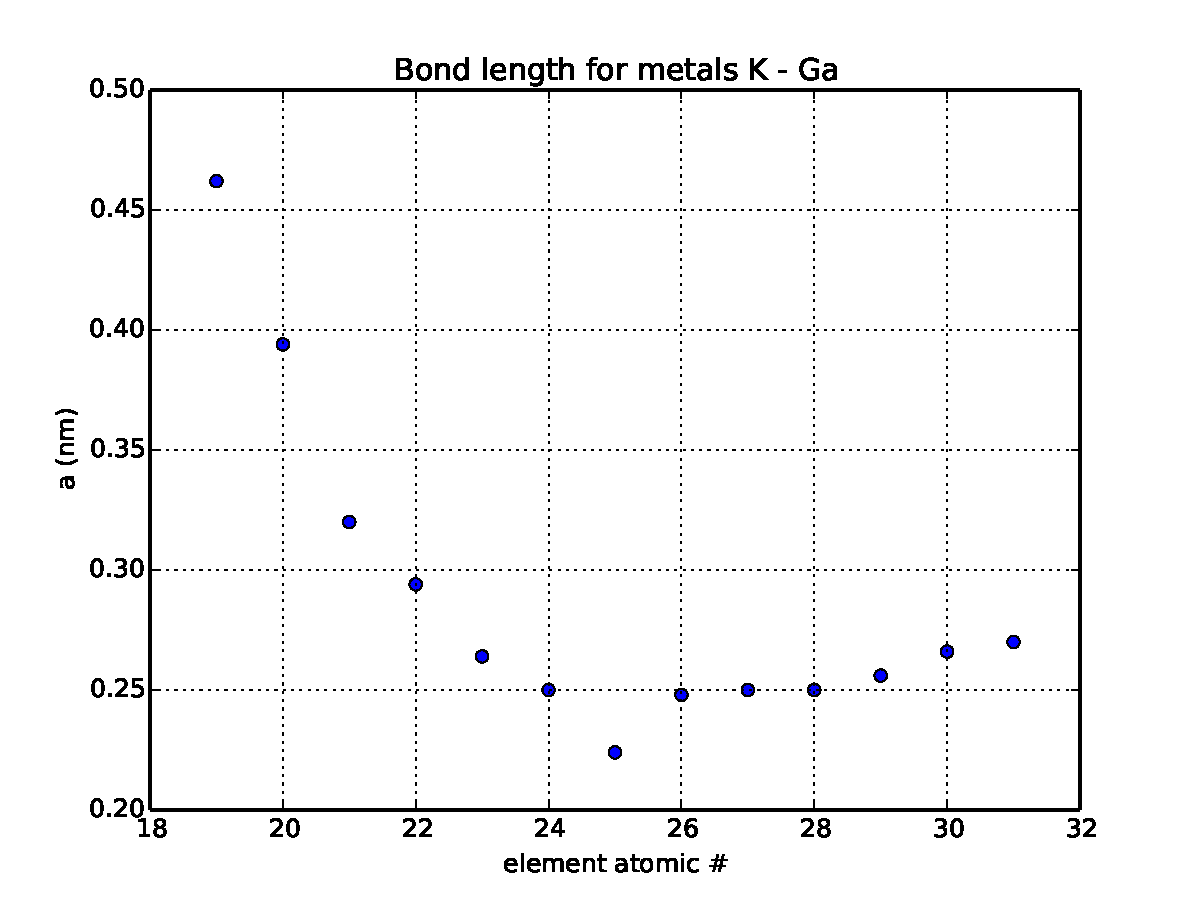
\includegraphics[width=250pt]{graph_p2_46.pdf}
\end{center}

\begin{problem}{2.52}
Due to its large atomic diameter, neon has a higher heat of solution in vitreous silica than helium. If the heat of solution of neon in vitreous silica is $-6.70$ kJ/mol and the solubility at $25\degree$C is $9.07 \e{23}$ atoms/($m^3$*atm), calculate the solubility at $200\degree$C. (See problem 2.51.)
\end{problem}
% --------------------------------------------------------------
%     You don't have to mess with anything below this line.
% --------------------------------------------------------------
 
\end{document}
